\documentclass{article}
\usepackage[T1]{fontenc}
\usepackage{lmodern}
\usepackage{graphicx}
\usepackage{amsmath,amssymb}
\usepackage[a4paper,margin=2cm]{geometry}
\usepackage[absolute,overlay]{textpos}
\setlength{\TPHorizModule}{1mm}
\setlength{\TPVertModule}{1mm}
\usepackage[indonesian]{babel}
\usepackage{hyperref}
\setlength{\emergencystretch}{2em}
% unit: Halaman 29

\begin{document}

% === Halaman 29 (llm) ===

\begin{itemize}
  \item Contoh: Misalkan $U = 1111$
\end{itemize}

Algoritma sederhana memperoleh \textit{keystream} di dalam \textit{keystream generator} misalnya adalah sebagai berikut:

\textcolor{red}{XOR-kan bit ke-1 dengan bit ke-4 dari empat bit sebelumnya:}

\vspace{10mm}

\textcolor{blue}{111101011001000}111101011... \quad 111101...

\vspace{5mm}

dan akan berulang setiap 15 bit.

\begin{itemize}
  \item Secara umum, jika panjang $U$ adalah $n$ bit, maka bit-bit kunci tidak akan berulang sampai $2^n - 1$ bit.
\end{itemize}

\[ 111101011001000 \]

% deskripsi: Ilustrasi operasi XOR antara bit pertama dan keempat dari rangkaian bit untuk menghasilkan bit berikutnya dalam keystream generator.
% bbox normalisasi: [0.5600, 0.4500, 0.6400, 0.6100]
\begin{textblock*}{16.80mm}(117.60mm,133.65mm)
\noindent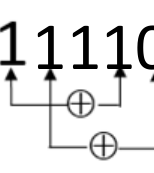
\includegraphics[width=16.80mm,height=47.52mm]{../../images/llm/page_029_img_01.png}%
\end{textblock*}

\end{document}
